\section{Generalised tangent method}
\label{sec:proof_generalised_tangent}
\begin{figure}[htbp]
    \centering
    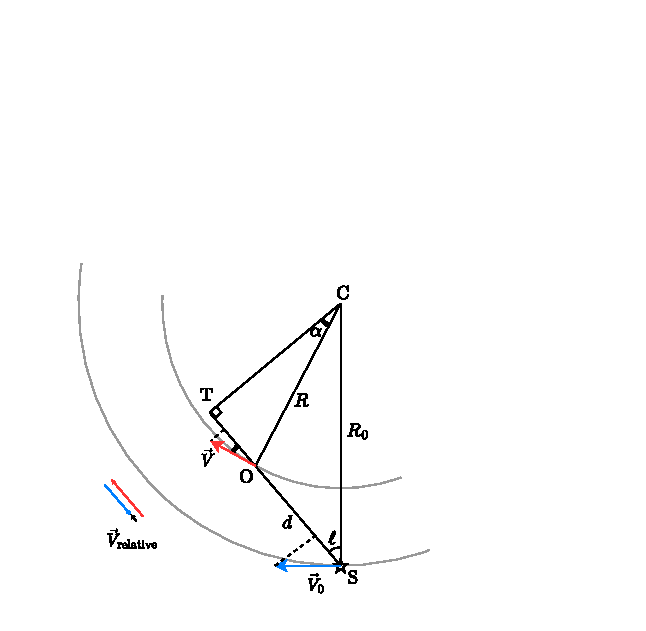
\includegraphics[width=0.5\textwidth]{figures/inner_circle_method.pdf}
    \caption{Schematic of the inner circle method}
    \label{fig:inner_circle_method}
\end{figure}
%
The velocity of the observed galactic object O given the relative velocity $V_r$ projected on the line of sight axis ST between the observer S and the object is given by
\begin{equation}
    V = \frac{R}{R_0} \left( \frac{V_r}{\sin(\ell)} + V_0 \right)
\end{equation}
\begin{proof}
    Using trigonometry, the distance TC can be written as
    \begin{equation}
       \textrm{TC} = R_0 \sin\ell = R \cos\alpha
       \label{eq:proof1}
    \end{equation}
    % and
    % \begin{equation}
    %     \textrm{TO} = R_0 \cos\ell - d = R \sin\alpha
    %    \label{eq:proof2}
    % \end{equation}
    The projected relative velocity is given by
    \begin{equation}
        V_r = V \cos\alpha - V_0 \sin\ell
       \label{eq:proof3}
    \end{equation}
    From \autoref{eq:proof1}, it is clear that $\cos\alpha = \frac{R_0}{R} \sin\ell$. Substituting in \autoref{eq:proof3}, we get
    \begin{equation}
        V_r = \left( \frac{R_0}{R} V - V_0 \right) \sin\ell
    \end{equation}
    By rearanging this equation, the final result can be found
    \begin{equation}
        V = \frac{R}{R_0} \left( \frac{V_r}{\sin(\ell)} + V_0 \right)
    \end{equation}
\end{proof}

\section{Oort constants method}
\label{sec:oort_method}

\begin{proof}
    Let $V_r$ and $V_t$ be the component along the line of sight and perpendicular to the line of sight of the relative velocity between the object and the observer $\vec V_\textrm{relative} = \vec V - \vec V_0$. From the Oort constants, the distance $d$ between the observer and the object is
    \begin{equation}
        d = \frac{V_r}{A \sin(2\ell)}
    \end{equation}
    Using the second Oort constant $B = \frac{V_r}{d} - A \cos(2\ell)$, the transverse component can be expressed as
    \begin{equation}
        V_t = d (B + A \cos(2\ell))
    \end{equation}
    To obtain the angular velocity of the object, the velocity of the observer, along and perpendicular to the line of sight, must simply be added to each component:
    \begin{multline}
        V_{\parallel} = V_r + V_0 \sin(\ell) \\
        V_{\perp} = V_t - V_0 \cos(\ell)
    \end{multline}
    The norm then gives the angular velocity:
    \begin{equation}
        \begin{aligned}
            V &= \sqrt{(V_r + V_0 \sin(\ell))^2 + (V_t - V_0 \cos(\ell))^2} \\
            &= \sqrt{(V_r + V_0 \sin(\ell))^2 + (d (B + A \cos(2\ell)) - V_0 \cos(\ell))^2}
        \end{aligned}
    \end{equation}
\end{proof}